% Source: Weinberg GR, physical PDF pp. 532--556
%         (printed pp. 506--528; boundary pages are partial).
%         Physical pp. 538/540 both reproduce printed p. 512, and physical
%         pp. 539/541 both reproduce printed p. 513; each repeated printed
%         leaf is transcribed once.
% Coverage: Section 15.5, The Cosmic Microwave Radiation Background;
%           equations (15.5.1)--(15.5.42), including all unnumbered displays.
% Figures/tables/footnotes: Figures 15.3--15.4; Tables 15.1--15.3;
%           reference notes 51--86 (including lettered supplements).
% Status: source-reviewed and compile-clean; visually proofed.
% Uncertainties: none.
% MODERNIZATION: source scale factor -> a(t), and source present-epoch scale
% factor -> a_0, with
% H=\dot a/a and the existing modern q convention. The source's radiation
% constant a is written a_{\mathrm{rad}} to avoid collision with the scale factor.
% The photon four-vector in the Doppler calculation is written time-first for
% the binding (-+++) metric; all resulting observable formulas are unchanged.
% LITERAL-OPERATOR AUDIT: every leading sign and continuation operator in
% equations (15.5.1)--(15.5.42), especially (15.5.3), (15.5.24), and the
% geodesic formulas (15.5.34)--(15.5.37), was checked against pp. 532--556.

\subsection{The Cosmic Microwave Radiation Background}\label{sec:15.5}

The Einstein field equations require that the scale factor \(a(t)\) must have
been extremely small at some finite time in the past (see
Section~\ref{sec:15.1}). At this early epoch, matter and radiation were
presumably in thermal equilibrium, with a very high temperature. As the
universe subsequently expanded, both radiation and matter cooled. Eventually,
when the temperature had dropped to about \(4000^\circ\mathrm{K}\), the free
electrons joined atoms, so that the opacity dropped sharply, breaking the
thermal contact between matter and radiation. Whatever radiation existed at
that time has since been enormously red-shifted, but it still fills the space
around us.

It is widely, though not unanimously, believed, that the microwave radiation
background discovered in 1965 is just this left-over radiation, red-shifted by
a factor of approximately 1500 since the universe became transparent. If so,
then the microwave background provides information of unparalleled value as
to the history of the universe, not only back to the time when electrons became
bound but, as we shall see, back much further, to the first few seconds of
cosmic history.

First, let us consider what sort of background radiation spectrum we would
expect on purely theoretical grounds. The proper energy density of the
left-over photons, with frequency at the present time \(t_0\) between \(\nu\)
and \(\nu+\dd\nu\), is given by Eq.~\eqref{eq:15.4.10} as
\begin{align}
  \rho_{\gamma0}(\nu)\dd\nu
  &=
  h\nu\,8\pi\nu^2\dd\nu
  \int_0^{t_0}
  \exp\left[-\frac{h\nu a_0}{kT(t)a(t)}\right]
  \notag\\
  &\qquad\times
  \Lambda\left(\nu\frac{a_0}{a(t)},t\right)
  P(t_0,t;\nu)\dd t,
  \tag{15.5.1}\label{eq:15.5.1}
\end{align}
where \(h\) is Planck's constant; \(k\) is Boltzmann's constant;
\(a_0\) is an abbreviation for \(a(t_0)\); \(T(t)\) is the temperature of
the matter (as opposed to the radiation) at time \(t\);
\(\Lambda(\nu,t)\) is the absorption rate for a photon of frequency \(\nu\)
at time \(t\); and \(P(t_0,t;\nu)\) is the probability, taking account of
stimulated emission, that a photon of frequency \(\nu a_0/a(t)\) present at
time \(t\) will survive until the present:
\begin{equation}
  P(t_0,t;\nu)
  =
  \exp\left\{
    -\int_t^{t_0}
    \left[
      1-\exp\left(
        -\frac{h\nu a_0}{kT(t')a(t')}
      \right)
    \right]
    \Lambda\left(\nu\frac{a_0}{a(t')},t'\right)\dd t'
  \right\}.
  \tag{15.5.2}\label{eq:15.5.2}
\end{equation}
The lower limit on the integral \eqref{eq:15.5.1} can be chosen as any time
\(t_1\) for which \(P(t_0,t_1;\nu)\) is negligible; surely the choice
\(t_1=0\) meets this requirement.

The formula \eqref{eq:15.5.1} can usefully be rewritten in the form
\begin{equation}
  \rho_{\gamma0}(\nu)\dd\nu
  =
  8\pi h\nu^3\dd\nu
  \int_0^{t_0}
  \left[
    \exp\left(\frac{h\nu a_0}{kT(t)a(t)}\right)-1
  \right]^{-1}
  \frac{\dd}{\dd t}P(t_0,t;\nu)\dd t.
  \tag{15.5.3}\label{eq:15.5.3}
\end{equation}
The survival probability \(P\) rises from \(P=0\) at \(t=0\) to \(P=1\)
at \(t=t_0\), so this is just a \emph{weighted average of Planck black-body
distributions}. If the opacity drops very steeply at some time \(t_R\), then
\(P\) is nearly a step function at \(t=t_R\), and \eqref{eq:15.5.3} gives
\begin{equation}
  \rho_{\gamma0}(\nu)\dd\nu
  \simeq
  \frac{8\pi h\nu^3\dd\nu}
  {\exp(h\nu/kT_{\gamma0})-1},
  \tag{15.5.4}\label{eq:15.5.4}
\end{equation}
where
\begin{equation}
  T_{\gamma0}
  \equiv
  \frac{T(t_R)a(t_R)}{a_0}.
  \tag{15.5.5}\label{eq:15.5.5}
\end{equation}
Thus, \emph{under the assumption of a sharp drop in opacity, the present
radiation background should have a black-body spectrum, with temperature
\(T_{\gamma0}\)}.

It is common to report measurements of the radiation background in terms of a
radiation flux \(\phi_{\gamma0}(\nu)\), the energy received per unit time, per
unit receiving area, per unit solid angle, and per unit frequency interval. The
flux can be calculated in c.g.s.\ units from the above formulas for
\(\rho_{\gamma0}(\nu)\) by using
\[
  \phi_{\gamma0}(\nu)=\frac{\rho_{\gamma0}(\nu)c}{4\pi}.
\]
The background measurements are also frequently reported in terms of an
\emph{equivalent black-body temperature} \(T_{\gamma0}(\nu)\), which is
defined to be that temperature for which black-body radiation would have the
observed energy density or flux at frequency \(\nu\). That is,
\begin{equation}
  \rho_{\gamma0}(\nu)\dd\nu
  \equiv
  \frac{8\pi h\nu^3\dd\nu}
  {\exp[h\nu/kT_{\gamma0}(\nu)]-1}.
  \tag{15.5.6}\label{eq:15.5.6}
\end{equation}
A black-body spectrum is then simply characterized as having
\(T_{\gamma0}(\nu)\) independent of \(\nu\). Finally, it is occasionally
convenient to report background measurements in terms of an \emph{antenna
temperature} \(T_A(\nu)\), which is defined to be that temperature for which
the low-frequency Rayleigh--Jeans approximation to \eqref{eq:15.5.4} would
give the observed density or flux at frequency \(\nu\):
\begin{equation}
  \rho_{\gamma0}(\nu)\dd\nu
  \equiv
  8\pi kT_A(\nu)\nu^2\dd\nu.
  \tag{15.5.7}\label{eq:15.5.7}
\end{equation}
Wherever possible, our discussion here will refer to the black-body temperature
\(T_{\gamma0}(\nu)\).

If we make no assumptions about the thermal history of matter before the drop
in opacity, then all we can say is that the radiation background should have
roughly a black-body spectrum, with a temperature that tells us the value of
\(a(t)/a_0\) at the time the universe became transparent. The theoretical
situation is tremendously improved if we can assume that, during the time that
matter and radiation were in thermal contact, the matter temperature relaxed
according to the formula
\begin{equation}
  T(t)=\frac{A}{a(t)},
  \tag{15.5.8}\label{eq:15.5.8}
\end{equation}
with \(A\) a constant. In this case, the first factor in the integrand of
\eqref{eq:15.5.3} can be taken outside the integral, so we get the black-body
formula \eqref{eq:15.5.4}, \emph{no matter how gradual is the transition from
an opaque to a transparent universe}. Further, by taking \(t_0\) in
\eqref{eq:15.5.3} to be an arbitrary time \(t\), we see now that
\(\rho_\gamma\) is given by a black-body formula
\begin{equation}
  \rho_\gamma(\nu,t)\dd\nu
  =
  \frac{8\pi h\nu^3\dd\nu}
  {\exp[h\nu/kT_\gamma(t)]-1},
  \tag{15.5.9}\label{eq:15.5.9}
\end{equation}
with
\begin{equation}
  T_\gamma(t)=\frac{A}{a(t)}
  \tag{15.5.10}\label{eq:15.5.10}
\end{equation}
at all times---after, during, and before the drop in opacity. It is of course
not surprising that the radiation would be described by the black-body formula
\eqref{eq:15.5.9} during the time that matter and radiation were in
equilibrium, and naturally its temperature \eqref{eq:15.5.10} equaled the
matter temperature \eqref{eq:15.5.8} during that time. The noteworthy thing
here is that the radiation goes on obeying the black-body formula
\eqref{eq:15.5.9}, with temperature given by \eqref{eq:15.5.10},
throughout the period of transition from high to low opacity, and thereafter
until the present. The constant \(A\) can be determined by setting \(t=t_0\)
in \eqref{eq:15.5.8}, so the radiation temperature at all times is
\begin{equation}
  T_\gamma(t)=T_{\gamma0}\left[\frac{a_0}{a(t)}\right],
  \tag{15.5.11}\label{eq:15.5.11}
\end{equation}
and the matter temperature during equilibrium is the same:
\begin{equation}
  T(t)=T_{\gamma0}\left[\frac{a_0}{a(t)}\right].
  \tag{15.5.12}\label{eq:15.5.12}
\end{equation}
Thus the present radiation temperature \(T_{\gamma0}\) determines the thermal
history of the early universe during the whole period when \(Ta\) was constant.

In order to see when \(Ta\) is likely to be constant, let us consider the model
of an ideal gas in equilibrium with black-body radiation. The energy density of
black-body radiation is given by integrating \eqref{eq:15.5.9} over \(\nu\):
\[
  \rho_\gamma(t)=a_{\mathrm{rad}}T_\gamma^4(t),
\]
where, in c.g.s.\ units,
\[
  a_{\mathrm{rad}}\equiv\frac{8\pi^5k^4}{15h^3c^3}
  =7.5641\times10^{-15}\,
  \mathrm{erg\,cm^{-3}\,deg^{-4}}.
\]
Thus the total pressure and energy density in this model are
\[
  p=nkT+\frac13a_{\mathrm{rad}}T^4,
  \qquad
  \rho=nm+(\gamma-1)^{-1}nkT+a_{\mathrm{rad}}T^4,
\]
where \(n\) is the number density of gas particles, \(m\) is their mass, and
\(\gamma\) is the specific heat ratio of the gas, equal to \(5/3\) for a
monatomic gas like atomic hydrogen. The equation of particle conservation can
be written
\begin{equation}
  na^3=n_0a_0^3,
  \tag{15.5.13}\label{eq:15.5.13}
\end{equation}
whereas the equation \eqref{eq:15.1.21} of energy conservation reads
\[
  \frac{\dd}{\dd a}
  \left[
    nma^3+(\gamma-1)^{-1}nkTa^3+a_{\mathrm{rad}}T^4a^3
  \right]
  =
  -3nkTa^2-a_{\mathrm{rad}}T^4a^2.
\]
Using \eqref{eq:15.5.13} and rearranging terms, this gives
\begin{equation}
  \frac{a}{T}\frac{\dd T}{\dd a}
  =
  -\left[
    \frac{\sigma+1}
    {\sigma+\tfrac13(\gamma-1)^{-1}}
  \right],
  \tag{15.5.14}\label{eq:15.5.14}
\end{equation}
where \(\sigma k\) is the \emph{photon entropy per gas particle}:
\begin{equation}
  \sigma
  \equiv
  \frac{4a_{\mathrm{rad}}T^3}{3nk}
  =
  74.0\,
  \frac{[T(\mathrm{deg})]^3}{n(\mathrm{cm^{-3}})}.
  \tag{15.5.15}\label{eq:15.5.15}
\end{equation}
For \(\sigma\ll1\), Eq.~\eqref{eq:15.5.14} gives
\begin{equation}
  T\propto a^{-3(\gamma-1)},
  \tag{15.5.16}\label{eq:15.5.16}
\end{equation}
which is just the usual temperature-volume relation for the adiabatic expansion
of an ideal gas. On the other hand, for \(\sigma\gg1\),
Eq.~\eqref{eq:15.5.14} gives
\begin{equation}
  T\propto a^{-1}.
  \tag{15.5.17}\label{eq:15.5.17}
\end{equation}

Even for large \(\sigma\), as matter goes out of equilibrium with radiation,
its temperature curve ultimately shifts from \eqref{eq:15.5.17} to
\eqref{eq:15.5.16}. However, if \(\sigma\) is extremely large, then as long
as there is any significant thermal contact between matter and radiation, the
radiation will continue to overpower the matter, and the matter temperature
will have the hoped-for behavior \eqref{eq:15.5.8}. In this case,
Eqs.~\eqref{eq:15.5.12}, \eqref{eq:15.5.13}, and \eqref{eq:15.5.15} give
\(\sigma\) constant:
\begin{equation}
  \sigma=\frac{4a_{\mathrm{rad}}T_{\gamma0}^3}{3n_0k}.
  \tag{15.5.18}\label{eq:15.5.18}
\end{equation}
Hence, if \(\sigma\) is ever very large, then it stays very large. We then say
that we are dealing with a \emph{hot universe}. In a hot universe, the
background radiation approximately satisfies \eqref{eq:15.5.9} and
\eqref{eq:15.5.11} at all times, and the matter temperature obeys
\eqref{eq:15.5.12} until the opacity becomes extremely small. Note that the
number density of photons in black-body radiation is the integral of
\(\rho_\gamma(\nu)/h\nu\) over \(\nu\), or
\[
  n_\gamma
  =
  \frac{30\zeta(3)}{\pi^4}\frac{a_{\mathrm{rad}}T_\gamma^3}{k}
  =
  0.37\frac{a_{\mathrm{rad}}T_\gamma^3}{k},
\]
so
\[
  \sigma=0.37\frac{n_{\gamma0}}{n_0},
\]
and the condition for a hot universe can be expressed as a requirement that
there are many photons for each proton or neutron in the present universe.
None of these considerations gives any clue as to the actual value of
\(T_{\gamma0}\), or even as to whether this is a hot universe.

The first theoretical estimate of the radiation temperature was based on a
theory of element synthesis worked out in the late 1940's by George Gamow and
his collaborators.\hyperref[ch15-ref-51]{\textsuperscript{51}} (This subject
will be discussed in greater detail in Section~\ref{sec:15.7}.) At the time
when the temperature was \(10^{9\circ}\mathrm{K}\), corresponding to the
dissociation temperature of deuterium, the number density of nucleons must have
been roughly \(10^{18}\,\mathrm{cm^{-3}}\), in order that a fraction of order
10 to 50\% of the neutrons and protons could fuse into heavier elements. The
specific photon entropy \eqref{eq:15.5.15} at that time was then
\(\sigma\simeq10^{11}\), so in this model the universe is indubitably hot,
and \(aT_\gamma\) would therefore have remained constant, both while the
universe remained opaque, and thereafter until the present. With a present
baryon number density \(10^{-6}\,\mathrm{cm^{-3}}\), the scale factor at
present must be larger than when \(T\simeq10^{9\circ}\mathrm{K}\) by a factor
\((10^{18}/10^{-6})^{1/3}\), or \(10^8\), so the present radiation
temperature should be \(10^{-8}\) times \(10^{9\circ}\mathrm{K}\), or roughly
\(10^\circ\mathrm{K}\). A somewhat more detailed analysis along these lines,
carried out in 1950 by Alpher and
Herman,\hyperref[ch15-ref-52]{\textsuperscript{52}} gave
\(T_{\gamma0}\simeq5^\circ\mathrm{K}\). Unfortunately, Alpher and Herman went
on to express doubts as to whether this radiation would have survived until the
present. It is of course true that the individual photons extant at
\(T\simeq10^{9\circ}\mathrm{K}\) would have been absorbed long before now.
However, because \(\sigma\gg1\), the matter temperature must relax like
\(a^{-1}\), so that the photons emitted just as the universe is becoming
transparent must have had the same value of \(Ta\) as during the time of
element synthesis. Nevertheless, the remarkable prediction of a
\(5^\circ\mathrm{K}\) black-body radiation background was allowed to slip
into obscurity.

The problem of determining \(T_{\gamma0}\) was taken up again in 1965 by
Dicke, Peebles, Roll, and
Wilkinson.\hyperref[ch15-ref-53]{\textsuperscript{53}} They argued that the
universe must once have been hotter than \(10^{10\circ}\mathrm{K}\), because
it either has expanded from a singularity with \(a=0\), or, if it undergoes a
cyclic oscillation between finite values of \(a\), it must get hot enough to
dissociate the heavy elements left over from the previous cycle. This argument
does not fix a value for the present radiation temperature, but Dicke et al.\
reasoned that the energy density of cosmic black-body radiation should not be
large enough to give \(q_0\gg1\) (see Section~\ref{sec:15.2}), so that
\(T_{\gamma0}\lesssim40^\circ\mathrm{K}\). The really important feature of
their work, however, was not this estimate, but rather the fact that at last
the black-body radiation background was being taken seriously, with an
experiment to measure \(T_{\gamma0}\) being prepared by Roll and Wilkinson.

The difficult part of measuring a radiation temperature less than
\(40^\circ\mathrm{K}\) is of course that the receiver circuits are at a much
higher temperature, so that the signal must be hundreds of times weaker than
the receiver noise. In order to pick out the signal, Roll and Wilkinson planned
to use a radiometer invented by Dicke in 1945. In this device the radio
receiver is switched back and forth a hundred times a second between one horn
pointing at the sky and another looking into a bath of liquid helium. The
receiver output is filtered to separate just that part that varies with a
frequency of 100 Hz, and the strength of this filtered output then measures the
difference between the radiation received from the liquid helium and the sky.

Before Roll and Wilkinson could complete a measurement of \(T_{\gamma0}\),
they learned that Penzias and
Wilson\hyperref[ch15-ref-54]{\textsuperscript{54}} had observed a weak
background signal at a radio wavelength \(\lambda=7.35\,\mathrm{cm}\) in the
large horn antenna at Holmdel, New Jersey, built to observe the Echo satellite.
The antenna temperature could be fit to the curve
\[
  T_A(\theta)=4.4^\circ\mathrm{K}
  +2.3^\circ\mathrm{K}\sec\theta,
\]
where \(\theta\) is the angle between the antenna axis and the zenith. The
thickness of atmosphere (taken as a flat slab) through which the antenna beam
passes is proportional to \(\sec\theta\), so the second term could be ascribed
to radiation from our atmosphere. An additional \(0.9^\circ\mathrm{K}\) was
estimated as the contribution of ohmic losses in the antenna and radiation
from the earth into the antenna side lobes, leaving for the cosmic microwave
background a net antenna temperature \(3.5^\circ\mathrm{K}\pm1^\circ
\mathrm{K}\). Since \(kT_A\gg h\nu\), this is also the equivalent black-body
temperature
\[
  T_{\gamma0}(7.35\,\mathrm{cm})
  =
  3.5^\circ\mathrm{K}\pm1^\circ\mathrm{K}.
\]
This observation, probably the most important to cosmology since Hubble's
discovery of the relation between red shift and distance, was
published\hyperref[ch15-ref-54]{\textsuperscript{54}} in 1965 under the
modest title ``A Measurement of Excess Antenna Temperature at 4080 MHz'' with
the paper by Dicke, Peebles, Roll, and
Wilkinson\hyperref[ch15-ref-53]{\textsuperscript{53}} appearing as a companion
article to explain the fundamental significance of this measurement.

\begingroup
\renewcommand{\thetable}{15.1}
\begin{table}[htbp]
  \centering
  \caption{Summary of Measurements of the Background Radiation Flux at
  Microwave and Far-Infrared Wavelengths. (The temperatures listed are those
  for which black-body radiation would give the observed flux at the indicated
  wavelength.)}
  \label{tab:15.1}
  \scriptsize
  \setlength{\tabcolsep}{3.5pt}
  \begin{tabular}{@{}rllc@{}}
    \toprule
    \(\lambda\) (cm) & Method & Reference & \(T_\gamma(\lambda)\)
    (\(^{\circ}\mathrm{K}\))\\
    \midrule
    73.5 & Ground-based radiometer & a & \(3.7\pm1.2\)\\
    49.2 & Ground-based radiometer & a & \(3.7\pm1.2\)\\
    21.0 & Ground-based radiometer & b & \(3.2\pm1.0\)\\
    20.7 & Ground-based radiometer & c & \(2.8\pm0.6\)\\
    7.35 & Ground-based radiometer & d & \(3.5\pm1.0\)\\
    3.2 & Ground-based radiometer & e & \(3.0\pm0.5\)\\
    3.2 & Ground-based radiometer & f & \(2.69^{+0.16}_{-0.21}\)\\
    1.58 & Ground-based radiometer & f & \(2.78^{+0.12}_{-0.17}\)\\
    1.50 & Ground-based radiometer & g & \(2.0\pm0.8\)\\
    0.924 & Ground-based radiometer & h & \(3.16\pm0.26\)\\
    0.856 & Ground-based radiometer & i & \(2.56^{+0.17}_{-0.22}\)\\
    0.82 & Ground-based radiometer & j & \(2.9\pm0.7\)\\
    0.358 & Ground-based radiometer & j\(^{\prime}\) & \(2.4\pm0.7\)\\
    0.33 & Ground-based radiometer & k & \(2.46^{+0.40}_{-0.44}\)\\
    0.33 & Ground-based radiometer & k\(^{\prime}\) & \(2.61\pm0.25\)\\
    0.263 & CN (\(J=1/J=0\)) & l & \(\lesssim2.3\)\\
    0.263 & CN (\(J=1/J=0\)) & m &
      \(3.22\pm0.15\ \zeta\mathrm{\ Oph};\ 3.0\pm0.6\ \zeta\mathrm{\ Per}\)\\
    0.263 & CN (\(J=1/J=0\)) & n & \(3.75\pm0.50\)\\
    0.263 & CN (\(J=1/J=0\)) & o & \(\leq2.82\)\\
    0.132 & CN (\(J=2/J=1\)) & n & \(<7.0\)\\
    0.132 & CN (\(J=2/J=1\)) & o & \(<4.74\)\\
    0.0559 & CH & n & \(<6.6\)\\
    0.0559 & CH & o & \(<5.43\)\\
    0.0359 & \(\mathrm{CH}^+\) & o & \(<8.11\)\\
    0.04--0.13 & Rocket-borne IR telescope & p & \(8.3^{+2.2}_{-1.3}\)\\
    \(>0.05\) & Balloon-borne IR radiometer & q &
      \(\simeq3.6,\ 5.5,\ 7.0\)\\
    0.6--0.008 & Rocket-borne IR radiometer & r & \(3.1^{+0.5}_{-2.0}\)\\
    0.18--1.0 & Balloon-borne IR radiometer & s & \(2.7^{+0.4}_{-0.2}\)\\
    0.13--1.0 & Balloon-borne IR radiometer & s & \(2.8\pm0.2\)\\
    0.09--1.0 & Balloon-borne IR radiometer & s & \(\leq2.7\)\\
    0.054--1.0 & Balloon-borne IR radiometer & s & \(\leq3.4\)\\
    \bottomrule
  \end{tabular}
\end{table}
\endgroup

\begingroup
\small
\setlength{\parindent}{0pt}
\textsuperscript{a} T.~F.~Howell and J.~R.~Shakeshaft, \emph{Nature}
\textbf{216}, 753 (1967).
\textsuperscript{b} A.~A.~Penzias and R.~W.~Wilson, \emph{Astron.\ J.}
\textbf{72}, 315 (1967).
\textsuperscript{c} T.~F.~Howell and J.~R.~Shakeshaft, \emph{Nature}
\textbf{210}, 1318 (1966).
\textsuperscript{d} A.~A.~Penzias and R.~W.~Wilson, \emph{Ap.\ J.}
\textbf{142}, 419 (1965).
\textsuperscript{e} P.~G.~Roll and D.~T.~Wilkinson, \emph{Phys.\ Rev.\
Letters} \textbf{16}, 405 (1966).
\textsuperscript{f} R.~A.~Stokes, R.~B.~Partridge, and D.~T.~Wilkinson,
\emph{Phys.\ Rev.\ Letters} \textbf{19}, 1199 (1967).
\textsuperscript{g} W.~J.~Welch, S.~Keachie, D.~D.~Thornton, and G.~Wrixon,
\emph{Phys.\ Rev.\ Letters} \textbf{18}, 1068 (1967).
\textsuperscript{h} M.~S.~Ewing, B.~F.~Burke, and D.~H.~Staelin,
\emph{Phys.\ Rev.\ Letters} \textbf{19}, 1251 (1967).
\textsuperscript{i} D.~T.~Wilkinson, \emph{Phys.\ Rev.\ Letters} \textbf{19},
1195 (1967).
\textsuperscript{j} Y.~I.~Puzanov, A.~E.~Salomonovich, and K.~S.~Starkovich,
\emph{Astron.\ Zh.} (USSR) \textbf{44}, 1128 (1967) [trans.\
\emph{Soviet A.\ J.} \textbf{11}, 905 (1968)].
\textsuperscript{j\(^{\prime}\)} A.~G.~Kislyakov, V.~I.~Chernyshev,
Yu.~V.~Lebskii, V.~A.~Mal'tsev, and N.~V.~Serov, \emph{Ast.\ Zh.}
\textbf{48}, 39 (1971) [transl.\ \emph{Sov.\ Astron.--AJ} \textbf{15}, 29
(1971)].
\textsuperscript{k} P.~E.~Boynton, R.~A.~Stokes, and D.~T.~Wilkinson,
\emph{Phys.\ Rev.\ Letters} \textbf{21}, 462 (1968).
\textsuperscript{k\(^{\prime}\)} M.~F.~Millea, M.~McColl, R.~J.~Pederson,
and F.~L.~Vernon, Jr., \emph{Phys.\ Rev.\ Letters} \textbf{26}, 919 (1971).
\textsuperscript{l} A.~McKellar, \emph{Publs.\ Dominion Astrophys.\
Observatory} (Victoria, B.C.) \textbf{7}, 251 (1941).
\textsuperscript{m} G.~B.~Field and J.~L.~Hitchcock, \emph{Phys.\ Rev.\
Letters} \textbf{16}, 817 (1966).
\textsuperscript{n} P.~Thaddeus and J.~F.~Clauser, \emph{Phys.\ Rev.\
Letters} \textbf{16}, 819 (1966).
\textsuperscript{o} V.~J.~Bortolot, J.~F.~Clauser, and P.~Thaddeus,
\emph{Phys.\ Rev.\ Letters} \textbf{22}, 307 (1969).
\textsuperscript{p} K.~Shivanandan, J.~R.~Houck, and M.~O.~Harwit,
\emph{Phys.\ Rev.\ Letters} \textbf{21}, 1460 (1968); J.~R.~Houck and
M.~Harwit, \emph{Ap.\ J.} \textbf{157}, L45 (1969). For a recalibration of
this data and further data see M.~Harwit, J.~R.~Houck, and R.~V.~Wagoner,
\emph{Nature} \textbf{228}, 451 (1970); J.~L.~Pipher, J.~R.~Houck,
B.~W.~Jones, and M.~Harwit, \emph{Nature} \textbf{231}, 375 (1971).
\textsuperscript{q} D.~Muehlner and R.~Weiss, \emph{Phys.\ Rev.\ Letters}
\textbf{24}, 742 (1970).
\textsuperscript{r} A.~G.~Blair, J.~G.~Beery, F.~Edeskuty, R.~D.~Hiebert,
J.~P.~Shipley, and K.~D.~Williamson, Jr., \emph{Phys.\ Rev.\ Letters}
\textbf{27}, 1154 (1971).
\textsuperscript{s} D.~Muehlner and R.~Weiss, to be published (1972).
\endgroup

Although Penzias and Wilson reported their result as an ``excess antenna
temperature,'' it is important to realize that they had only measured a
radiation flux at a single wavelength. It remained to verify the Planck form
\eqref{eq:15.5.4} of the radiation frequency distribution. In
Table~\ref{tab:15.1} I have listed the measurements of the equivalent
black-body temperature of the background radiation that have been carried out
at various microwave and far-infrared wavelengths.

At wavelengths above 100 cm, the cosmic background is swamped by the VHF
radiation emitted by our galaxy. In the range from 75 to 0.3 cm, the background
radiation can be measured with a ground-based microwave radiometer, like that
employed by Penzias and Wilson and Roll and Wilkinson. However, below
\(\lambda=3\,\mathrm{cm}\) the emission from our atmosphere becomes extremely
troublesome, and it is necessary to make observations at mountain altitudes,
and at wavelengths, such as 0.9 cm and 0.3 cm, where ``windows'' appear in the
atmosphere. Below \(\lambda=0.3\,\mathrm{cm}\) there are no more useful
windows, and the measuring equipment must be carried on a balloon or a rocket.
In addition, it is possible to infer a background temperature at certain
wavelengths from the absorption of light by molecules in interstellar space.
For instance, cyanogen has a visible absorption line at
\(3874\,\text{\AA}\), corresponding to transitions from the ground electronic
configuration to an excited electronic configuration. (See
Figure~\ref{fig:15.3}.)

Both electronic configurations are split into rotational energy levels,
distinguished by the rotational angular momentum \(J\), so this absorption line
splits into a number of components,\hyperref[ch15-ref-55]{\textsuperscript{55}}
of which the most important are
\(R(0)\,[J=0\to J=1;\ \lambda=3874.608\,\text{\AA}]\),
\(R(1)\,[J=1\to J=2;\ \lambda=3873.998\,\text{\AA}]\),
\(P(1)\,[J=1\to J=0;\ \lambda=3875.763\,\text{\AA}]\), and
\(R(2)\,[J=2\to J=3;\ \lambda=3873.369\,\text{\AA}]\). (These transitions
are governed by a dipole selection rule, \(\Delta J=\pm1\).) In 1941
McKellar\hyperref[ch15-ref-56]{\textsuperscript{56}} discovered that cyanogen
radicals in an interstellar cloud between us and the star \(\zeta\) Ophiuchi
were absorbing light from that star, not only in the \(R(0)\) transition from
the \(J=0\) ground state, but also in the \(R(1)\) transition from the first
excited rotational state, which is at an excitation energy corresponding to a
wavelength 2.64 mm. From the relative strength of the two absorption lines, a
population for the \(J=1\) state could be inferred, corresponding to a
temperature \(2.3^\circ\mathrm{K}\). McKellar could not be sure that there was
not some special excitation mechanism at work, so the only conclusion that
could be reached was that the radiation background at
\(\lambda=2.64\,\mathrm{mm}\) has an equivalent black-body temperature less
than about \(2.3^\circ\mathrm{K}\). After the discovery of
\(3.5^\circ\mathrm{K}\) radiation at 7.35 cm by Penzias and
Wilson,\hyperref[ch15-ref-54]{\textsuperscript{54}}
Field,\hyperref[ch15-ref-57]{\textsuperscript{57}}
Woolf,\hyperref[ch15-ref-58]{\textsuperscript{58}} and
Shklovsky\hyperref[ch15-ref-58a]{\textsuperscript{58a}} independently
realized that McKellar's old observations of \(\zeta\) Ophiuchi might actually
have measured the radiation background temperature, and not just set an upper
bound on it.

\begingroup
\renewcommand{\thefigure}{15.3}
\begin{figure}[htbp]
  \centering
  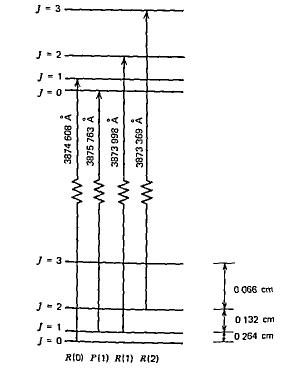
\includegraphics[width=0.48\textwidth]{figures/chapter15/fig15-03.png}
  \caption{Transitions in the cyanogen absorptive spectrum used to set limits
  on the cosmic microwave radiation background.}
  \label{fig:15.3}
\end{figure}
\endgroup


This was confirmed by theoretical
analyses\hyperref[ch15-ref-57]{\textsuperscript{57},}\hyperref[ch15-ref-59]{\textsuperscript{59}}
that rejected all other rotational excitation mechanisms, and the measurements
were repeated, now including data\hyperref[ch15-ref-60]{\textsuperscript{60}}
on the \(P(1)\) absorption line, and from a number of other stars. No precise
radiation temperature has emerged from these measurements, but it appears
pretty certain that \(T_\gamma\) at 2.64 mm is between 2.7 and
\(3.7^\circ\mathrm{K}\). There has also been an unsuccessful
search\hyperref[ch15-ref-60]{\textsuperscript{60}} for the \(R(2)\) absorption
line in CN and various absorption lines from excited rotational states in CH
and \(\mathrm{CH}^+\), which allows upper limits to be set on \(T_\gamma\) at
wavelengths 1.32 mm, 0.559 mm, and 0.359 mm.

Inspection of Table~\ref{tab:15.1} shows that with the exception of the rocket
and balloon infrared measurements, all observations are consistent with a
\(2.7^\circ\mathrm{K}\) black-body distribution. But before we conclude that
a black-body distribution has been definitely established, we have to ask how
significant this agreement is, and we have to worry about the high-altitude
infrared measurements. All of the data at wavelengths above 1 cm unfortunately
lie in that part of a \(2.7^\circ\mathrm{K}\) Planck distribution that is very
well approximated by the Rayleigh--Jeans law
\begin{equation}
  \rho_{\gamma0}(\nu)\dd\nu
  \simeq
  8\pi kT_{\gamma0}\nu^2\dd\nu,
  \tag{15.5.19}\label{eq:15.5.19}
\end{equation}
which can be obtained by letting \(\nu\to0\) in Eq.~\eqref{eq:15.5.4}. For
instance, at \(\lambda=1.5\,\mathrm{cm}\), the flux for a
\(2.7^\circ\mathrm{K}\) black body is only 15\% below what would be given by
the Rayleigh--Jeans formula \eqref{eq:15.5.19}, and even at
\(\lambda=0.856\,\mathrm{cm}\), the Planck flux is only 35\% below the
Rayleigh--Jeans flux. (See Figure~\ref{fig:15.4}.)

\begingroup
\renewcommand{\thefigure}{15.4}
\begin{figure}[htbp]
  \centering
  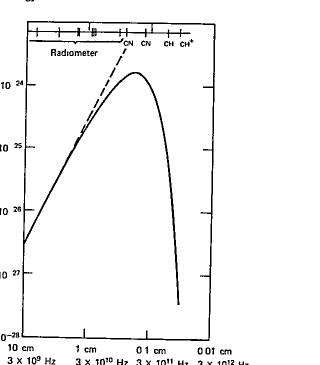
\includegraphics[width=0.58\textwidth]{figures/chapter15/fig15-04.png}
  \caption{Energy density per frequency interval for
  \(2.7^\circ\mathrm{K}\) black-body radiation. The solid curve gives the
  Planck spectrum \eqref{eq:15.5.4}; the dashed line gives the
  Rayleigh--Jeans spectrum \eqref{eq:15.5.7} for an antenna temperature of
  \(2.7^\circ\mathrm{K}\). The short vertical lines mark frequencies at which
  the black-body temperature has been measured or bounded by radiometer or
  interstellar absorption observations.}
  \label{fig:15.4}
\end{figure}
\endgroup


This is a serious deficiency, because one can imagine a number of models that
would give a Rayleigh--Jeans curve \eqref{eq:15.5.19} down to wavelengths
well below the point where the Planck law begins to drop below the
Rayleigh--Jeans law. For instance, suppose that the observed microwave
background was emitted at a time \(t_R\) when the photon absorption probability
\(1-P\) dropped sharply, not from 1 to 0, but from some value
\(\alpha<1\) to 0. Then instead of a black-body law,
Eq.~\eqref{eq:15.5.3} would give a \emph{gray-body law},
\begin{equation}
  \rho_{\gamma0}(\nu)\dd\nu
  =
  \frac{8\pi\alpha h\nu^3\dd\nu}
  {\exp(h\nu/kT_1)-1},
  \tag{15.5.20}\label{eq:15.5.20}
\end{equation}
with \(0<\alpha<1\) and \(T_1=T(t_R)a(t_R)/a(t_0)\). Then, to account for
the data at \(\lambda>1\,\mathrm{cm}\), it would be necessary to take
\[
  T_1\simeq\frac{2.7^\circ\mathrm{K}}{\alpha},
\]
and the flux would then be given by the Rayleigh--Jeans law down to a
wavelength \(\lambda\simeq\alpha\,\mathrm{cm}\). The total radiant energy
density must be less than \(10^{-7}\,\mathrm{erg/cm^3}\) (see
Section~\ref{sec:15.2}), so \(\alpha\) could in principle be as small as
0.08. In order to rule out this sort of theory, we must use data for
\(\lambda<1\,\mathrm{cm}\), and preferably for \(\lambda<0.2\,\mathrm{cm}\),
where a \(2.7^\circ\mathrm{K}\) Planck distribution has its maximum.
Unfortunately, these are just the wavelengths where the atmosphere begins to
interfere with radiometer measurements. The whole case for a black-body
distribution, rather than a gray-body distribution, therefore rests on the
radiometer measurements\hyperref[ch15-ref-61]{\textsuperscript{61}} at
mountain altitude, which give a flux at \(\simeq3\,\mathrm{mm}\) three times
less than expected for the Rayleigh--Jeans law
[Eq.~\eqref{eq:15.5.19} with \(T_{\gamma0}=2.7^\circ\mathrm{K}\)], plus the
absorption spectra of interstellar molecules, which give upper
limits\hyperref[ch15-ref-62]{\textsuperscript{62}} on the flux, at 2.63 mm,
1.32 mm, 0.559 mm, and 0.359 mm, less than Rayleigh--Jeans by factors 2.9,
2.2, 12, and 9.3, respectively. This evidence points strongly to a
distribution that does not keep going up like the Rayleigh--Jeans law, but
bends over steeply around 0.2 cm, as expected for black-body radiation.

However, this simple picture is contradicted by some of the data taken in the
far-infrared by rocket- and balloon-borne equipment. These measurements are
essentially bolometric; what is observed is the total power per unit area and
solid angle received by detectors having various complicated spectral-response
functions. Initially the rocket observations at
Cornell\hyperref[ch15-ref-63]{\textsuperscript{63}} and the balloon
observations at M.I.T.\hyperref[ch15-ref-64]{\textsuperscript{64}} both
indicated a flux many times larger than expected at these wavelengths for a
\(2.7^\circ\mathrm{K}\) black-body background. Indeed, taken together with the
interstellar absorption measurements, these data were not consistent with any
smooth spectral distribution, let alone a Planck or Rayleigh--Jeans
distribution. The Cornell measurements have since been
recalibrated\hyperref[ch15-ref-64a]{\textsuperscript{64a}} and
repeated,\hyperref[ch15-ref-64b]{\textsuperscript{64b}} and now indicate a
much smaller flux, but the flux is still two orders of magnitude greater than
expected for a \(2.7^\circ\mathrm{K}\) Planck distribution. However, other
rocket observations\hyperref[ch15-ref-64c]{\textsuperscript{64c}} and new
balloon observations by the M.I.T.\
group\hyperref[ch15-ref-64d]{\textsuperscript{64d}} give results consistent
with a \(2.7^\circ\mathrm{K}\) background. These discrepancies might perhaps
arise from a number of strong lines superimposed on a
\(2.7^\circ\mathrm{K}\) background, or might be due to unexpected sources of
atmospheric radiation at high altitudes. These uncertainties will probably be
with us until far-infrared measurements can be made with cryogenic equipment
carried by artificial satellites.

In checking the agreement of the observed flux of background radiation at
various wavelengths with the Planck formula, it is useful to keep in mind the
departures from this formula that may be expected on theoretical grounds, even
if the observed microwave radiation represents a cosmic background left over
from the early universe. With a black-body temperature
\(T_{\gamma0}=2.7^\circ\mathrm{K}\), the specific photon entropy
\eqref{eq:15.5.15} is \(\sigma=1.35\times10^8\) for a present mass density
\(n_0m_N=1.8\times10^{-29}\,\mathrm{g/cm^3}\), or
\(\sigma=5.4\times10^9\) for
\(n_0m_N=4.5\times10^{-31}\,\mathrm{g/cm^3}\). As we have seen, these high
\(\sigma\) values lead us to expect that the matter temperature \(T\) would
have followed the radiation temperature \(T_\gamma\propto a^{-1}\) as long as
there was any appreciable thermal contact between matter and radiation. This
expectation is borne out by detailed calculations by Peebles of recombination
in a universe filled with ionized
hydrogen.\hyperref[ch15-ref-65]{\textsuperscript{65}} For a present density
\(n_0m_N=1.8\times10^{-29}\,\mathrm{g/cm^3}\), the fractional ionization
dropped sharply from 99.8\% at \(T_\gamma=5000^\circ\mathrm{K}\) to 0.98\%
at \(T_\gamma=3000^\circ\mathrm{K}\), and then to 0.0053\% at
\(T_\gamma=1500^\circ\mathrm{K}\). However, even though the mean free path of
photons at these low ionization levels was very long, the matter temperature
when \(T_\gamma=2000^\circ\mathrm{K}\) was \(T=1920^\circ\mathrm{K}\), and
at \(T_\gamma=1500^\circ\mathrm{K}\), \(T=1280^\circ\mathrm{K}\). For
smaller values of the present mass density, \(T\) followed \(T_\gamma\) even
more closely. In consequence, the departures from a Planck distribution should
be quite small. According to Peebles, the largest effects are the excess of
photons left over from the \(2p\to1s\) Lyman \(\alpha\) transition and the
\(2s\to1s\) two-photon transition, by which the recombined hydrogen atoms
reached their ground states. These photons now show up red-shifted by a factor
of order \(>1000\) from
\(\lambda(\text{Lyman }\alpha)=1215\,\text{\AA}\) and
\(\lambda(2\gamma)\simeq2500\,\text{\AA}\), and thus produce departures from
a Planck distribution at wavelengths shorter than 0.015 mm. Unfortunately, at
these short wavelengths the cosmic radiation background is much less intense
than the radiation from interstellar
dust\hyperref[ch15-ref-66]{\textsuperscript{66}} and
gas\hyperref[ch15-ref-67]{\textsuperscript{67}} in our galaxy, so it is
unlikely that we shall be able to observe these departures from a black-body
spectral distribution.

There is one other important possible source of departures from the Planck
spectrum. The calculations of Peebles\hyperref[ch15-ref-65]{\textsuperscript{65}}
show that by the time the radiation temperature dropped to
\(200^\circ\mathrm{K}\), the residual hydrogen ionization was extremely small,
of order \(10^{-4}\) to \(10^{-5}\). However, the experiment on Lyman
\(\alpha\) absorption discussed in the last section shows that there cannot
have been any appreciable amount of neutral hydrogen since a time when
\(T_\gamma\simeq8^\circ\mathrm{K}\), corresponding to \(z\simeq2\). If there
really is a good deal of intergalactic hydrogen gas, as indicated by
measurements of \(q_0\) (see Section~\ref{sec:15.2}), then somehow or other
this hydrogen must have been reionized at a time when \(T_\gamma\) was between
\(4000^\circ\mathrm{K}\) and \(8^\circ\mathrm{K}\). If the reionization was
very early, then thermal contact would have been reestablished between matter
and radiation, and the Planck spectrum would have been distorted by an
increase in the individual photon energies. According to
Sunyaev,\hyperref[ch15-ref-68]{\textsuperscript{68}} the agreement between the
observed background radiation spectrum with the Planck formula already shows
that the reionization could not have occurred until \(T_\gamma\) dropped to
about \(800^\circ\mathrm{K}\).

There is also a great deal to be learned from the distribution of the
microwave background in angle. If this radiation really is left over from an
earlier period when matter and radiation were in thermal equilibrium, then we
should expect the radiation flux to be isotropic. However, there might be
anisotropies of small angular scale, owing to inhomogeneities in the primordial
plasma, possibly associated with the presence of nascent
galaxies.\hyperref[ch15-ref-66]{\textsuperscript{66}} (See
Section~\ref{sec:15.8}.) There might also be anisotropies of larger angular
scale, owing to a departure of the universe as a whole or our local
gravitational field\hyperref[ch15-ref-69]{\textsuperscript{69}} from perfect
isotropy, and there certainly is a small anisotropy with a \(360^\circ\)
angular scale owing to the motion of the solar system relative to the radiation
background. If the radiation background does not come from an earlier period
of thermal equilibrium, then its angular distribution may reveal its source;
for instance, if the radiation comes from a large number of discrete sources,
then we should find large anisotropies of very small angular scale, whereas if
it comes from our own galaxy, then we should expect a large-scale anisotropy
correlated with galactic latitude.

In looking for \emph{anisotropies of small angular scale}, a large antenna
pointed at a fixed angle relative to the earth is swept across the sky by the
rotation of the earth. If no special care is taken to maintain a stable
calibration, then the measured antenna temperature will show a gradual drift in
time, which does not concern us here. There will also be a small fluctuation
around this general drift, characterized by an r.m.s.\ fluctuation value
\((\Delta T_A)_{\mathrm{obs}}\). If there really is an intrinsic fluctuation
\(\Delta T_A\) with an angular scale \(\theta\) comparable with the beam width
\(B\), then \((\Delta T_A)^2_{\mathrm{obs}}\) will be given by
\((\Delta T_A)^2\) plus a term arising from noise in the receiver, so that
\begin{equation}
  \Delta T_A\lesssim(\Delta T_A)_{\mathrm{obs}}
  \qquad\text{for }\theta\simeq B.
  \tag{15.5.21}\label{eq:15.5.21}
\end{equation}
On the other hand, if the intrinsic fluctuation scale \(\theta\) is much less
than the beam width \(B\), then the beam can be regarded as split into \(N\)
patches of angular diameter \(\theta\), where
\[
  N\simeq\left(\frac{B}{\theta}\right)^2.
\]
The fluctuation \(\Delta P\) in the power \(P\) from each patch is given by
\eqref{eq:15.5.7} as
\[
  \frac{\Delta P}{P}\simeq\frac{\Delta T_A}{T_A}.
\]
The total power received is \(NP\), but the fluctuations have random sign,
and so the r.m.s.\ fluctuation in the total power is \(N^{1/2}\Delta P\).
Taking account of receiver noise, the observed relative fluctuation in
received power will be greater than \(N^{1/2}\Delta P/NP\), so
\[
  \frac{(\Delta T_A)_{\mathrm{obs}}}{T_A}
  \gtrsim
  N^{-1/2}\frac{\Delta P}{P}
  \simeq
  N^{-1/2}\frac{\Delta T_A}{T_A},
\]
and therefore
\begin{equation}
  \Delta T_A
  \lesssim
  N^{1/2}(\Delta T_A)_{\mathrm{obs}}
  \simeq
  \left(\frac{B}{\theta}\right)(\Delta T_A)_{\mathrm{obs}}
  \qquad\text{for }\theta\ll B.
  \tag{15.5.22}\label{eq:15.5.22}
\end{equation}
A more detailed analysis\hyperref[ch15-ref-70]{\textsuperscript{70}} shows
that for fluctuations of arbitrary angular scale \(\theta\)
\[
  \Delta T_A
  \leq
  \left[1+\frac{B^2}{\theta^2}\right]^{1/2}
  (\Delta T_A)_{\mathrm{obs}},
\]
in agreement with \eqref{eq:15.5.21} and \eqref{eq:15.5.22}. For a very
strong intrinsic fluctuation with \(\Delta T_A\simeq T_A\),
Eq.~\eqref{eq:15.5.22} sets an upper limit on the angular scale
\begin{equation}
  \theta_{\max}
  \simeq
  \frac{B(\Delta T_A)_{\mathrm{obs}}}{T_A}.
  \tag{15.5.23}\label{eq:15.5.23}
\end{equation}
Measurements of \((\Delta T_A)_{\mathrm{obs}}\) at various wavelengths and
beam widths are listed in Table~\ref{tab:15.2}. The anisotropy is evidently
less than a few percent on any angular scale larger than a few seconds of arc.

\begingroup
\renewcommand{\thetable}{15.2}
\begin{table}[htbp]
  \centering
  \caption{Summary of Measurements of Fluctuations in the Microwave
  Background of Small Angular Scale.}
  \label{tab:15.2}
  \scriptsize
  \setlength{\tabcolsep}{4pt}
  \begin{tabular}{@{}cccccl@{}}
    \toprule
    \(\lambda\) (cm) & \(T_A\) (\(^{\circ}\mathrm K\)) & \(B\) &
    \((\Delta T_A)_{\mathrm{obs}}\) (\(^{\circ}\mathrm K\)) &
    \(\theta_{\max}\) & Reference\\
    \midrule
    7.35 & 2.56 & \(40'\) & 0.006 & \(5''\) & a\\
    3.95 & 2.50 & \(1.4'\times20'\) & 0.0007 & \(0.1''\) & a\(^{\prime}\)\\
    2.80 & 2.45 & \(1^\circ\) & 0.051 & \(75''\) & b\\
    2.80 & 2.45 & \(6^\circ\) & 0.036 & --- & b\\
    2.80 & 2.45 & \(10'\) & 0.0061 & \(1.5''\) & c\\
    2.80 & 2.45 & \(2^\circ\) & 0.0017 & --- & c\\
    0.35 & 1.14 & \(\simeq75''\) & 0.024 & \(1.6''\) & d\\
    0.35 & 1.14 & \(80''\)--\(100''\) & 0.008 & \(0.7''\) & d\(^{\prime}\)\\
    0.34 & 1.11 & \(12.5'\) & 0.2 & --- & e\\
    \bottomrule
  \end{tabular}

  \vspace{0.5em}
  \begin{minipage}{0.95\textwidth}
    Here \(\lambda\) is the wavelength, \(T_A\) is the antenna temperature
    for \(2.70^\circ\mathrm K\) black-body radiation, \(B\) is the beam width,
    \((\Delta T_A)_{\mathrm{obs}}\) is the observed r.m.s.\ fluctuation in antenna
    temperature, and \(\theta_{\max}\) is the largest angular scale at which
    the observations would allow gross anisotropies [see
    Eq.~\eqref{eq:15.5.23}]. The ``beam widths'' of \(1^\circ\), \(2^\circ\),
    and \(6^\circ\) were synthesized by integration of data obtained with a
    \(10'\) beam width. The measurement of \(\Delta T_A\) at 0.34 cm really is
    a measure of the change in slope of \(T_A(\theta)\) over an angular
    interval \(12.5'\).

    \textsuperscript{a} A.~A.~Penzias and R.~W.~Wilson, \emph{Ap.\ J.}
    \textbf{142}, 419 (1965).
    \textsuperscript{a\(^{\prime}\)} Yu.~N.~Pariskii and T.~B.~Pyatunina,
    \emph{Astron.\ Zh.} \textbf{47}, 1337 (1970) [transl.\ \emph{Sov.\
    Astron.--AJ} \textbf{14}, 1067 (1971)].
    \textsuperscript{b} E.~K.~Conklin and R.~N.~Bracewell, \emph{Phys.\ Rev.\
    Letters} \textbf{18}, 614 (1967).
    \textsuperscript{c} E.~K.~Conklin and R.~N.~Bracewell, \emph{Nature}
    \textbf{216}, 777 (1967).
    \textsuperscript{d} A.~A.~Penzias, J.~Schraml, and R.~W.~Wilson,
    \emph{Ap.\ J.} \textbf{157}, L49 (1969).
    \textsuperscript{d\(^{\prime}\)} P.~Boynton and R.~B.~Partridge, private
    communication.
    \textsuperscript{e} E.~E.~Epstein, \emph{Ap.\ J.} \textbf{148}, L157
    (1967).
  \end{minipage}
\end{table}
\endgroup

In searching for \emph{anisotropies of large angular scale}, it is not
necessary to use a large antenna, but care must be taken to maintain a stable
receiver calibration as the antenna beam is swept across the sky by the
rotation of the earth. In the work of Partridge and
Wilkinson,\hyperref[ch15-ref-71]{\textsuperscript{71}} this is managed by
aiming the horn so that it points near the celestial equator, and then for 15
min in each half-hour, inserting a vertical reflector that aims the beam toward
the north celestial pole. With and without the reflector, the angle between the
antenna beam and the vertical is the same (\(48^\circ\)), so the effects of
heating of the atmosphere, as well as of the apparatus, should be the same.
However, when the reflector is absent, the beam is scanned across the celestial
equator as the earth turns, whereas with the reflector inserted, the beam
points toward a more or less fixed point on the celestial sphere. Hence any
change with time in the \emph{difference} between the radiation flux received
with and without the reflector should be a measure of an intrinsic variation
of the flux with right ascension (i.e., azimuth) near the celestial equator.
This variation must have a 24-hr sidereal period, so it can be
Fourier-analyzed into components with periods \(24/n\) hr, where \(n\) is any
integer.

Measurements of the anisotropy are summarized in Table~\ref{tab:15.3}. There
is evidently no statistically significant anisotropy observed, and the maximum
change in \(T_{\gamma0}\) around the sky is probably less than 1\%.

\begingroup
\renewcommand{\thetable}{15.3}
\begin{table}[htbp]
  \centering
  \caption{Summary of Measurements of Anisotropies of Large Angular Scale in
  the Microwave Background. (The data used in reference e include those used
  in reference d.) All values of \(\Delta T_\gamma/T_{\gamma0}\) are based on
  an assumed value \(T_{\gamma0}=2.7^\circ\mathrm K\).}
  \label{tab:15.3}
  \small
  \begin{tabular}{@{}cccc@{}}
    \toprule
    \(\lambda\) (cm) & Type & \(\Delta T_\gamma/T_{\gamma0}\) (\%) &
    Reference\\
    \midrule
    7.35 & r.m.s. & \(\leq10\) & a\\
    7.35 & r.m.s. & \(\leq3.7\) & b\\
    3.75 & 24 hr & \(0.06\pm0.03\) & c\\
    3.2 & 12 hr & \(0.18\pm0.08\) & d\\
    3.2 & 24 hr & \(0.03\pm0.08\) & d\\
    3.2 & 12 hr & \(0.06\pm0.06\) & e\\
    3.2 & 24 hr & \(0.04\pm0.06\) & e\\
    0.8 & 12 hr & \(0.20\pm0.24\) & f\\
    0.8 & 24 hr & \(0.28\pm0.43\) & f\\
    \bottomrule
  \end{tabular}

  \vspace{0.5em}
  \begin{minipage}{0.92\textwidth}
    \scriptsize
    \textsuperscript{a} A.~A.~Penzias and R.~W.~Wilson, \emph{Ap.\ J.}
    \textbf{142}, 419 (1965).
    \textsuperscript{b} R.~W.~Wilson and A.~A.~Penzias, \emph{Science}
    \textbf{156}, 1100 (1967).
    \textsuperscript{c} E.~K.~Conklin, \emph{Nature} \textbf{222}, 971
    (1969).
    \textsuperscript{d} R.~B.~Partridge and D.~T.~Wilkinson, \emph{Phys.\
    Rev.\ Letters} \textbf{18}, 557 (1967).
    \textsuperscript{e} D.~T.~Wilkinson and R.~B.~Partridge, quoted by
    R.~B.~Partridge, \emph{American Scientist} \textbf{57}, 37 (1969).
    \textsuperscript{f} S.~P.~Boughn, D.~M.~Fram, and R.~B.~Partridge,
    \emph{Ap.\ J.} \textbf{165}, 439 (1971).
  \end{minipage}
\end{table}
\endgroup

The upper limits in the 24-hr component of the anisotropy
\(\Delta T_\gamma/T_{\gamma0}\) are particularly interesting, because they
set stringent upper limits on the velocity of the solar system relative to the
rest of the universe. Suppose that there is a fundamental reference frame in
which the background radiation is perfectly isotropic, with a Planck spectrum,
and assume that the earth moves with a velocity \(\mathbf v_\oplus\) with
respect to this fundamental frame. In the fundamental frame, the photons
within a solid angle \(\sin\theta\dd\theta\dd\phi\) and a frequency interval
\(\dd\nu\) contribute to the energy-momentum tensor an amount
\begin{align*}
  \dd T^{\mu\nu}
  &=
  \left(\frac{p^\mu p^\nu}{h^2\nu^2}\right)
  \left(\frac{\sin\theta\dd\theta\dd\phi}{4\pi}\right)
  \rho_{\gamma0}(\nu)\dd\nu
  \\
  &=
  2p^\mu p^\nu h^{-1}
  [e^{h\nu/kT_{\gamma0}}-1]^{-1}
  \sin\theta\dd\theta\dd\phi\,\nu\dd\nu,
\end{align*}
where, in time-first notation for the binding signature, \(p^\mu\) is the
photon momentum four-vector
\[
  p^\mu
  =
  h\nu(1,\sin\theta\cos\phi,\sin\theta\sin\phi,\cos\theta).
\]
(It follows from Eq.~\eqref{eq:2.8.4} that \(\dd T^{\mu\nu}\) is proportional
to \(p^\mu p^\nu\); the coefficient of \(p^\mu p^\nu\) is determined so that
the integral of \(\dd T^{00}\) over \(\theta\) and \(\phi\) should be
\(\rho_{\gamma0}\dd\nu\).) In the earth frame these photons have an
energy-momentum tensor given by the tensor transformation rule
\[
  \dd T'^{\mu\nu}
  =
  \Lambda^\mu{}_\rho\Lambda^\nu{}_\sigma\dd T^{\rho\sigma},
\]
where \(\Lambda\) is the Lorentz transformation defined by
Eqs.~\eqref{eq:2.1.17}--\eqref{eq:2.1.21}, taking
\(\mathbf v=-\mathbf v_\oplus\). In order to express \(\dd T'^{\mu\nu}\) in
terms of earth-frame quantities, we note that
\[
  p'^\mu=\Lambda^\mu{}_\nu p^\nu,
\]
or, taking the \(z\)-axis in the direction of the earth's velocity,
\[
  \nu'
  =
  \nu\frac{1-v_\oplus\cos\theta}{(1-v_\oplus^2)^{1/2}},
  \qquad
  \cos\theta'
  =
  \frac{-v_\oplus+\cos\theta}{1-v_\oplus\cos\theta},
  \qquad
  \phi'=\phi,
\]
where \(\theta\) is now the angle between the velocities of the earth and
photon. The solid angle then has the transformation rule
\[
  \sin\theta'\dd\theta'\dd\phi'
  =
  \left(\frac{\nu}{\nu'}\right)^2
  \sin\theta\dd\theta\dd\phi,
\]
and so the differential energy-momentum tensor in the earth frame is
\begin{align*}
  \dd T'^{\mu\nu}
  &=
  2p'^\mu p'^\nu h^{-1}
  [e^{h\nu/kT_{\gamma0}}-1]^{-1}
  \sin\theta\dd\theta\dd\phi\,\nu\dd\nu
  \\
  &=
  2p'^\mu p'^\nu h^{-1}
  [e^{h\nu'/kT'_{\gamma0}}-1]^{-1}
  \sin\theta'\dd\theta'\dd\phi'\,\nu'\dd\nu',
\end{align*}
where
\begin{equation}
  T'_{\gamma0}
  =
  \left(\frac{\nu'}{\nu}\right)T_{\gamma0}
  =
  (1-v_\oplus^2)^{-1/2}
  (1-v_\oplus\cos\theta)T_{\gamma0}.
  \tag{15.5.24}\label{eq:15.5.24}
\end{equation}
We see that \(\dd T'^{\mu\nu}\) has the same form as \(\dd T^{\mu\nu}\), so
that \emph{the background radiation in the earth frame has a Planck spectrum,
but with an angle-dependent temperature \(T'_{\gamma0}\)}. For
\(v_\oplus\ll1\), the departure of the measured temperature from the ``true''
black-body temperature \(T_{\gamma0}\) is
\begin{equation}
  \Delta T_{\gamma0}
  \simeq
  -v_\oplus\cos\theta\,T_{\gamma0}.
  \tag{15.5.25}\label{eq:15.5.25}
\end{equation}
In the experiments of Partridge and Wilkinson and of Conklin, the antenna
beam scans a circle on the celestial sphere of fixed declination \(\delta\)
once a day, so \(\Delta T_{\gamma0}\) should have a 24-hr period, with maximum
value given by
\begin{equation}
  \frac{(\Delta T_{\gamma0})_{\max}}{T_{\gamma0}}
  \simeq
  \frac{v_\oplus(\delta)}{c},
  \tag{15.5.26}\label{eq:15.5.26}
\end{equation}
where \(v_\oplus(\delta)\) is the component of the earth's velocity (in
c.g.s.\ units) along the cone of declination \(\delta\). This maximum is
attained when the antenna points in the azimuthal direction toward which the
earth is moving. The combined data of Partridge and
Wilkinson\hyperref[ch15-ref-71]{\textsuperscript{71}} give as a most likely
velocity \(v_\oplus(0^\circ)\simeq120\,\mathrm{km/sec}\) with a direction
toward 0 hr right ascension and a vector error of magnitude 180 km/sec.
Conklin\hyperref[ch15-ref-72]{\textsuperscript{72}} gives as a most likely
velocity \(v_\oplus(32^\circ\mathrm N)\simeq160\,\mathrm{km/sec}\) with a
direction toward 13 hr right ascension (just the opposite to Partridge and
Wilkinson!) and a vector error of magnitude 85 km/sec. It is reasonable to
conclude from these two results that
\begin{equation}
  \lvert\mathbf v_\oplus\rvert\lesssim300\,\mathrm{km/sec}.
  \tag{15.5.27}\label{eq:15.5.27}
\end{equation}
This upper limit is already of the same order of magnitude as the velocity of
the solar system in the local group of galaxies (owing mostly to the rotation
of our own galaxy) which is
estimated\hyperref[ch15-ref-73]{\textsuperscript{73}} as 315 km/sec toward
22 hr right ascension. Clearly neither the earth, nor the whole local group of
galaxies, is moving at great velocity relative to the radiation background. It
will be of very great interest to learn how fast we are moving, and in what
direction.

Apart from the effects of the earth's motion or local gravitational fields,
the microwave background might also exhibit anisotropies owing to a cosmic
inhomogeneity at the time \(t_R\) that the radiation was last emitted or
scattered. If there has been no scattering of the background radiation since
the recombination of hydrogen at about \(4000^\circ\mathrm{K}\), then the time
\(t_R\) corresponds to a red shift \(z_R\) given by
\[
  1+z_R
  \equiv
  \frac{a_0}{a(t_R)}
  =
  \frac{T_\gamma(t_R)}{T_{\gamma0}}
  \simeq
  \frac{4000^\circ\mathrm{K}}{2.7^\circ\mathrm{K}}
  =
  1500.
\]
On the other hand, if there is an intergalactic free-electron gas with number
density \(1.2\times10^{-5}/\mathrm{cm^3}\), then, as remarked in the last
section, the time of last scattering would correspond to a red shift
\(z_R\simeq6\). It would be very interesting to use the observed isotropy or
anisotropy of the present microwave background to determine the scales of
distances at which the universe is homogeneous or inhomogeneous at the time
\(t_R\).

To this end, consider two photons that leave comoving sources \(A\) and \(B\)
at time \(t_R\), and arrive at the earth at time \(t_0\), traveling along
paths separated at the earth by an angle \(\theta\). With the earth taken as
the origin, Eq.~\eqref{eq:14.3.1} gives the radial coordinates of the sources
\(A\) and \(B\) as
\begin{equation}
  r_A=r_B=r_1,
  \tag{15.5.28}\label{eq:15.5.28}
\end{equation}
where
\begin{equation}
  \int_0^{r_1}\frac{\dd r}{\sqrt{1-kr^2}}
  =
  \int_{t_R}^{t_0}\frac{\dd t}{a(t)}.
  \tag{15.5.29}\label{eq:15.5.29}
\end{equation}
Since photons travel to the earth on trajectories with constant direction
\(\mathbf x/r\), the sources will be separated in the Robertson--Walker
coordinate system by exactly the observed angle \(\theta\) that separates the
light rays arriving at the earth. That is,
\begin{equation}
  \frac{\mathbf x_A\cdot\mathbf x_B}{r_1^2}=\cos\theta,
  \tag{15.5.30}\label{eq:15.5.30}
\end{equation}
with the scalar product defined in terms of the Robertson--Walker coordinates
\(x^i\) as if these coordinates were Cartesian:
\begin{align}
  \mathbf x_A\cdot\mathbf x_B
  &\equiv
  x_A^1x_B^1+x_A^2x_B^2+x_A^3x_B^3
  \notag\\
  &=
  r_Ar_B
  [\sin\theta_A\sin\theta_B\cos(\phi_A-\phi_B)
  +\cos\theta_A\cos\theta_B].
  \tag{15.5.31}\label{eq:15.5.31}
\end{align}
Our problem is to determine the proper distance along a geodesic from \(A\)
to \(B\) at time \(t_R\) as a function of \(\theta\), for various assumed
values of \(z_R\) ranging from 6 to 1500.

According to Eq.~\eqref{eq:14.4.3}, the geodesic from \(A\) to \(B\) can be
chosen (setting \(\mathbf x_1\) equal to a vector \(a\mathbf e\) normal to
\(\mathbf n\)) to have the form
\begin{equation}
  \mathbf x(p)
  =
  \mathbf n p+a\mathbf e(1-kp^2)^{1/2},
  \tag{15.5.32}\label{eq:15.5.32}
\end{equation}
where \(a\) is a constant, \(p\) is a variable parameter, and \(\mathbf n\)
and \(\mathbf e\) are orthogonal unit vectors,
\begin{equation}
  \mathbf n\cdot\mathbf e=0,
  \qquad
  \mathbf n^2=\mathbf e^2=1,
  \tag{15.5.33}\label{eq:15.5.33}
\end{equation}
the scalar products being defined as in Eq.~\eqref{eq:15.5.31}. The initial
and final values of \(p\) are \(-p_1\) and \(+p_1\), with \(p_1\) determined
by the condition \eqref{eq:15.5.28}, that is,
\[
  r_1^2
  =
  \lvert\mathbf x(\pm p_1)\rvert^2
  =
  p_1^2+a^2(1-kp_1^2).
\]
In addition, the condition \eqref{eq:15.5.30} gives
\[
  \cos\theta
  =
  \frac{\mathbf x(+p_1)\cdot\mathbf x(-p_1)}{r_1^2}
  =
  \frac{-p_1^2+a^2(1-kp_1^2)}{r_1^2}.
\]
Both \(p_1\) and \(a\) can thus be expressed in terms of \(r_1\) and
\(\theta\):
\[
  p_1=r_1\sin\frac{\theta}{2},
  \qquad
  a=r_1\cos\frac{\theta}{2}
  \left[
    1-kr_1^2\sin^2\frac{\theta}{2}
  \right]^{-1/2}.
\]
The proper distance from \(A\) to \(B\) can now be calculated by integrating
the Robertson--Walker line element from \(-p_1\) to \(+p_1\):
\[
  d(\theta)
  =
  a(t_R)
  \int_{-p_1}^{p_1}
  \left\{
    \left\lvert\frac{\dd\mathbf x(p)}{\dd p}\right\rvert^2
    +
    \frac{k[\mathbf x(p)\cdot\dd\mathbf x(p)/\dd p]^2}
    {1-k\lvert\mathbf x(p)\rvert^2}
  \right\}^{1/2}\dd p,
\]
and thus
\begin{equation}
  d(\theta)
  =
  \frac{2a_0}{1+z_R}
  \int_0^{r_1\sin(\theta/2)}
  \frac{\dd p}{\sqrt{1-kp^2}}.
  \tag{15.5.34}\label{eq:15.5.34}
\end{equation}

If the time \(t_R\) of last scattering or emission occurs after the start of
the matter-dominated era, then \eqref{eq:15.2.5} and \eqref{eq:15.3.23} can
be used to express \(a_0\) and \(r_1\) in terms of \(H_0\), \(q_0\), and
\(z_R\), and we find
\begin{align}
  d(\theta)
  &=
  \frac{2}{H_0(1+z_R)\sqrt{2q_0-1}}
  \notag\\
  &\quad\times
  \sin^{-1}\left\{
    \frac{
      \sqrt{2q_0-1}
      [z_Rq_0+(q_0-1)(-1+\sqrt{2q_0z_R+1})]
    }{q_0^2(1+z_R)}
    \sin\frac{\theta}{2}
  \right\},
  \quad q_0>\frac12,\ k=+1,
  \tag{15.5.35}\label{eq:15.5.35}\\
  d(\theta)
  &=
  \frac{4}{H_0(1+z_R)}
  [1-(1+z_R)^{-1/2}]
  \sin\frac{\theta}{2},
  \quad q_0=\frac12,\ k=0,
  \tag{15.5.36}\label{eq:15.5.36}\\
  d(\theta)
  &=
  \frac{2}{H_0(1+z_R)\sqrt{1-2q_0}}
  \notag\\
  &\quad\times
  \sinh^{-1}\left\{
    \frac{
      \sqrt{1-2q_0}
      [z_Rq_0+(q_0-1)(-1+\sqrt{2q_0z_R+1})]
    }{q_0^2(1+z_R)}
    \sin\frac{\theta}{2}
  \right\},
  \quad q_0<\frac12,\ k=-1.
  \tag{15.5.37}\label{eq:15.5.37}
\end{align}
In particular, for \(\theta\to0\),
Eqs.~\eqref{eq:15.5.35}--\eqref{eq:15.5.37} give
\[
  d(\theta)
  \longrightarrow
  \frac{
    [z_Rq_0+(q_0-1)(-1+\sqrt{2q_0z_R+1})]\theta
  }{
    q_0^2(1+z_R)^2H_0
  }
  \qquad\text{for }\theta\to0.
\]

If the homogeneity of the universe is achieved by the physical transport of
energy and momentum from one place to another at velocities less than that of
light, then we should expect\hyperref[ch15-ref-74]{\textsuperscript{74}} the
universe at time \(t_R\) to be inhomogeneous over distances larger than twice
the ``particle horizon'' \eqref{eq:15.3.32}, because no homogenizing signal
could travel from any point to a pair of comoving particles separated by a
proper distance greater than \(2d_H(t_R)\) by time \(t_R\). If this is
correct, then the microwave background ought to exhibit large anisotropies for
angular scales greater than an angle \(\theta_H\), which can be calculated by
equating \(2d_H(t_R)\), given by Eq.~\eqref{eq:15.3.33}, to
\(d(\theta_H)\), given by Eqs.~\eqref{eq:15.5.35}--\eqref{eq:15.5.37}:
\begin{equation}
  \sin\frac{\theta_H}{2}
  =
  \frac{q_0\sqrt{2q_0z_R+1}}
  {z_Rq_0+(q_0-1)(-1+\sqrt{2q_0z_R+1})}.
  \tag{15.5.38}\label{eq:15.5.38}
\end{equation}
If \(z_R\simeq1500\), then we can use the approximation
\begin{equation}
  \theta_H
  \simeq
  2\left(\frac{2q_0}{z_R}\right)^{1/2}
  \simeq
  4.2^\circ\sqrt{q_0}.
  \tag{15.5.39}\label{eq:15.5.39}
\end{equation}
(This result would not be very much changed if the matter-dominated era began
somewhat after the recombination of hydrogen.) If \(z_R\simeq6\) and
\(q_0=\tfrac12\) or \(q_0=1\), then \(\theta_H\simeq75^\circ\). However,
there is no sign of any appreciable anisotropy in the microwave background at
such angular scales---on the contrary, the microwave radiation appears to be
highly isotropic on all angular scales greater than \(1^\circ\). In the light
of the above analysis, it is difficult to understand how such a high degree of
isotropy could be produced by any physical process occurring at any time since
the initial singularity.

The observed distributions of the radiation background in frequency and angle
certainly suggest that this is isotropic black-body radiation left over from an
earlier period when matter and radiation were in thermal equilibrium. However,
other possibilities are not yet excluded by the data. The energy density of
starlight within our galaxy is of the order of
\(5\times10^{-13}\,\mathrm{erg/cm^3}\), just about the same as the energy
density of \(2.7^\circ\mathrm{K}\) black-body radiation. For this reason,
Hoyle, Narlikar, and
Wickramasinghe\hyperref[ch15-ref-75]{\textsuperscript{75}} have suggested
that a large fraction of the optical-frequency starlight in our own and other
galaxies may be absorbed by interstellar grains, which are heated to a few
degrees, and reemit the energy at microwave frequencies, either as a continuum
or in discrete lines. It would not be impossible for this reemitted radiation
to be isotropic and to imitate a Planck spectrum, but this seems artificial.
Another possibility that has been widely considered is that the microwave
background may arise from a large number of discrete
sources.\hyperref[ch15-ref-76]{\textsuperscript{76}} Here again, a Planck
spectrum would not be impossible over the accessible range of wavelengths, but
there is no special reason to expect it. Also, in this case the observed
isotropy does put severe limits on any discrete source theory. For example, if
the microwave background comes from discrete sources at an average distance of
order \(H_0^{-1}\), then we should expect gross anisotropies in the microwave
background at an angular scale \(\theta\) such that the volume
\(H_0^{-3}\theta^2\) contains about one source, that is, for
\begin{equation}
  H_0^{-3}\theta^2d^{-3}\simeq1,
  \tag{15.5.40}\label{eq:15.5.40}
\end{equation}
where \(d\) is the mean separation of the sources. The limit
\(\theta\lesssim1\) sec given in Table~\ref{tab:15.2} thus sets an upper
limit \(\dd\lesssim1\,\mathrm{Mpc}\), about the same as the mean separation of
galaxies. Detailed analyses\hyperref[ch15-ref-77]{\textsuperscript{77}} of the
data in specific models show a density even greater than that of galaxies,
which would seem to rule out such theories.

The most interesting effects of the cosmic radiation background occur at early
times, when the temperature was much greater than at present. These effects
will be the subject of the next six sections. However, even at present, the
radiation background can have some interesting effects:

\emph{(A)} A relativistic electron of energy \(\gamma_em_e\) will undergo
inverse Compton scattering on the microwave photons, producing recoil photons
of average energy\hyperref[ch15-ref-78]{\textsuperscript{78}}
\begin{equation}
  \overline E
  =
  3.6\gamma_e^2kT_{\gamma0}
  =
  8.4\times10^{-4}\gamma_e^2\,\mathrm{eV}
  \left(\frac{T_{\gamma0}}{2.7^\circ\mathrm{K}}\right).
  \tag{15.5.41}\label{eq:15.5.41}
\end{equation}
Hoyle\hyperref[ch15-ref-79]{\textsuperscript{79}} proposed that inverse
Compton scattering of cosmic-ray electrons within our galaxy is responsible
for the diffuse background\hyperref[ch15-ref-13]{\textsuperscript{13}} of
cosmic X rays, but it was pointed out by
Gould\hyperref[ch15-ref-80]{\textsuperscript{80}} that the intensity from
this mechanism is several hundred times smaller than the observed X-ray
background. Soon after, Felton\hyperref[ch15-ref-81]{\textsuperscript{81}}
showed that the inverse Compton scattering of cosmic-ray electrons in
intergalactic space could produce X rays of the observed intensity. This model
has received support from the remark of Brecher and
Morrison,\hyperref[ch15-ref-82]{\textsuperscript{82}} that an observed kink
in the cosmic-ray electron spectrum at \(\gamma_e\simeq7\times10^3\) would,
according to \eqref{eq:15.5.41}, produce a kink in the spectrum of the diffuse
X-ray background at about 40 keV, just where a kink is
observed.\hyperref[ch15-ref-13]{\textsuperscript{13}} However, the more recent
calculations discussed in the last section indicate that this kink is due to
thermal bremsstrahlung in hot intergalactic hydrogen, with inverse Compton
scattering important only below 1 keV. The range of high-energy electrons in a
\(2.7^\circ\mathrm{K}\) background drops sharply for \(\gamma_e\gtrsim10^4\),
so if cosmic-ray electrons really come to us across intergalactic space, the
observed electron energy spectrum should be cut off sharply at energies above
10 GeV.

\emph{(B)} It has been observed\hyperref[ch15-ref-83]{\textsuperscript{83}}
that the very strong radio galaxy Centaurus A emits X rays in a frequency
range 1 to 10 keV with a total power
\(L_x=(11\pm4)\times10^{40}\,\mathrm{erg/sec}\). By using the theory of
synchrotron emission to account for the observed radio flux, it is
estimated\hyperref[ch15-ref-84]{\textsuperscript{84}} that Centaurus A
contains about \(1.7\times10^{59}\) ergs in cosmic-ray electrons, typically
with \(\gamma_e\simeq2.5\times10^3\). The inverse Compton scattering of these
electrons on a \(2.7^\circ\mathrm{K}\) radiation background would produce
X rays, at an average energy given by \eqref{eq:15.5.41} as 5 keV, with a
total power \(L_x\simeq5\times10^{40}\,\mathrm{erg/sec}\), in agreement with
the observed value. The most important aspect of this result is that the
predicted X-ray power is most sensitive to the background radiation flux at
short wavelengths, so that if the early
rocket\hyperref[ch15-ref-63]{\textsuperscript{63}} and
balloon\hyperref[ch15-ref-64]{\textsuperscript{64}} observations really gave
the correct temperature at these wavelengths, the X-ray power from Centaurus A
would be more than an order of magnitude larger than observed. However, this
interpretation of the Cen A X-ray source is still in doubt.

\emph{(C)} When a particle of mass \(m\) and momentum \(p\) strikes a photon
of energy \(w\) at an angle \(\theta\), the total energy in the
center-of-mass system is
\begin{align}
  E_c^2
  &=
  \left(w+\sqrt{p^2+m^2}\right)^2
  -(p^2+2pw\cos\theta+w^2)
  \notag\\
  &=
  2w\left[\sqrt{p^2+m^2}-p\cos\theta\right]+m^2.
  \tag{15.5.42}\label{eq:15.5.42}
\end{align}
In order for a nucleon to have a cross-section on a photon that is of first
rather than second order in \(\alpha=1/137\), it is necessary for \(E_c\) to
be greater than the threshold \(m_N+m_\pi\) for the process
\(\gamma+N\to\pi+N\):
\[
  \sqrt{p^2+m^2}-p\cos\theta
  \geq
  \frac{m_\pi^2+2m_Nm_\pi}{2w}
  \simeq
  \frac{m_Nm_\pi}{w}.
\]
Thus we expect a sharp
cutoff\hyperref[ch15-ref-85]{\textsuperscript{85}} in the cosmic-ray proton
energy spectrum at
\[
  E_{p,\max}
  \simeq
  \frac{m_Nm_\pi}{kT_{\gamma0}}
  \simeq
  3\times10^{20}\,\mathrm{eV},
\]
which is just about at the upper limit of current cosmic-ray observations.
Similarly, for cosmic-ray photons, the pair-production process
\(\gamma+\gamma\to e^++e^-\) gives a sharp
drop\hyperref[ch15-ref-86]{\textsuperscript{86}} in \(\gamma\)-ray range for
\(\sqrt{E_c^2}>2m_e\), that is, at an energy
\[
  E_{\gamma,\max}
  \simeq
  \frac{2m_e^2}{kT_{\gamma0}}
  \simeq
  10^{15}\,\mathrm{eV}.
\]
These upper limits apply only if we assume that the high-energy cosmic-ray
photons and protons arise outside our own galaxy.

It is not yet certain that the observed microwave background really is
black-body radiation left over from an earlier era. However, the case for this
view is certainly good enough to warrant a thorough examination of its
implications for the early universe. We now turn to a consideration of these
consequences.
